%\documentclass[xcolor=dvipsnames]{beamer}
%
%\usecolortheme[named=Blue]{structure}
%\setbeamertemplate{itemize items}[circle]
%
%\usepackage{smartdiagram}

\documentclass[xcolor=dvipsnames]{beamer}

\usecolortheme[named=Blue]{structure}
\setbeamertemplate{itemize items}[circle]

\usepackage{smartdiagram}


\author{Dr. Paul Larsen}
\date{\today}


\title{Artificial Intelligence for Finance and Insurance}
%\author{Dr. Paul Larsen}
%\date{\today}
\begin{document}
\maketitle

%%%%%%%%%%%%
% AI Does Note Exist
%%%%%%%%%%%%
\begin{frame}[c]
%\frametitle{'}
\begin{center}
\huge Artificial Intelligence Does Not Exist
\end{center}
\end{frame}

\begin{frame}
\frametitle{Artificial Intelligence Does Not Exist, But ...}
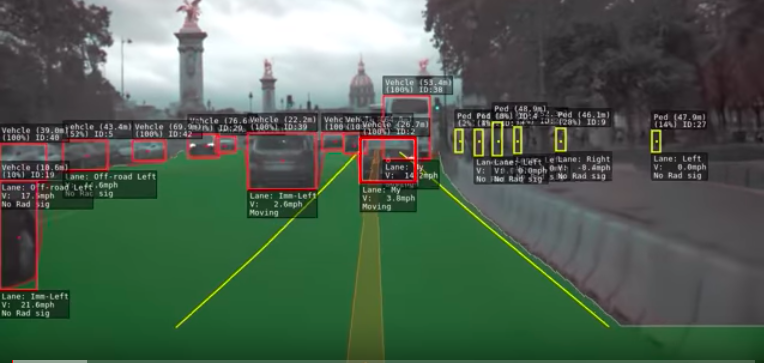
\includegraphics[width=\textwidth]{figures/tesla_paris}

Source: \href{https://www.youtube.com/watch?v=_1MHGUC_BzQs}{YouTube: greentheonly, Paris streets in the eyes of Tesla Autopilot}
\end{frame}

\begin{frame}
\frametitle{Artificial Intelligence Does Not Exist, But ...}
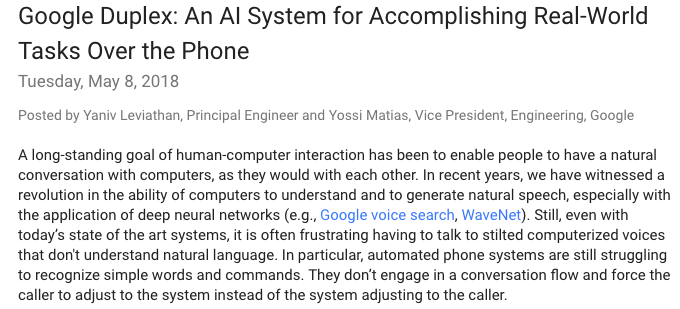
\includegraphics[width=\textwidth]{figures/google_duplex}

Source: \href{https://ai.googleblog.com/2018/05/duplex-ai-system-for-natural-conversation.html}{Google AI Blog}
\end{frame}

\begin{frame}
\frametitle{Artificial Intelligence Does Not Exist, But ...}
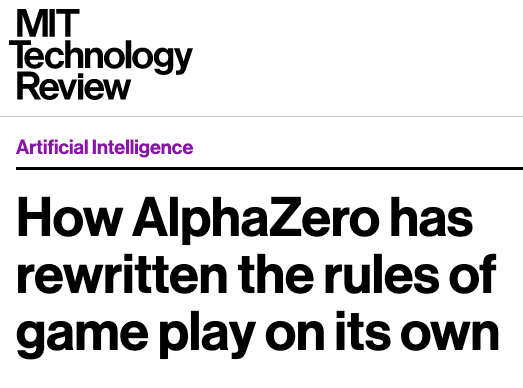
\includegraphics[width=0.8\textwidth]{figures/alpha_go}

Source: \href{https://www.technologyreview.com/s/612923/how-alphazero-has-rewritten-the-rules-of-gameplay-on-its-own/}{MIT Technology Review}
\end{frame}

\begin{frame}
\frametitle{AI Struggles With Context}
The scientist named the population, after their distinctive horn, Ovid’s Unicorn. These four-horned, silver-white unicorns were previously unknown to science.
Source: \href{https://www.lesswrong.com/posts/4AHXDwcGab5PhKhHT/humans-who-are-not-concentrating-are-not-general}{https://www.lesswrong.com/posts/4AHXDwcGab5PhKhHT/humans-who-are-not-concentrating-are-not-general}
\end{frame}

\begin{frame}
\frametitle{AI Struggles With Bias}
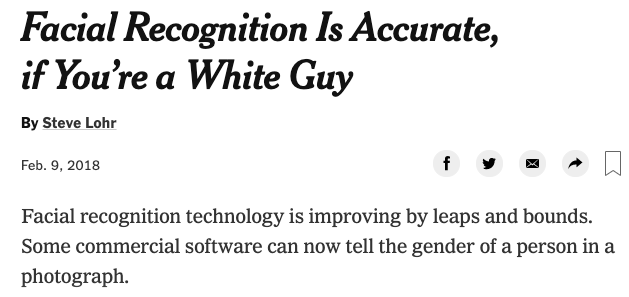
\includegraphics[width=\textwidth]{figures/facial_bias}

Source: \href{https://www.nytimes.com/2018/02/09/technology/facial-recognition-race-artificial-intelligence.html}{New York Times}

See also: \href{https://www.theverge.com/2018/1/12/16882408/google-racist-gorillas-photo-recognition-algorithm-ai}{James Vincent, The Verge, Google 'fixed' its racist algorithm by removing gorillas from its image-labeling tech}
\end{frame}


\begin{frame}
\frametitle{AI Struggles With Human Behavior}
\href{run:figures/siri_smart_sarcasm.m4a}{Siri Compliments}

\begin{center}
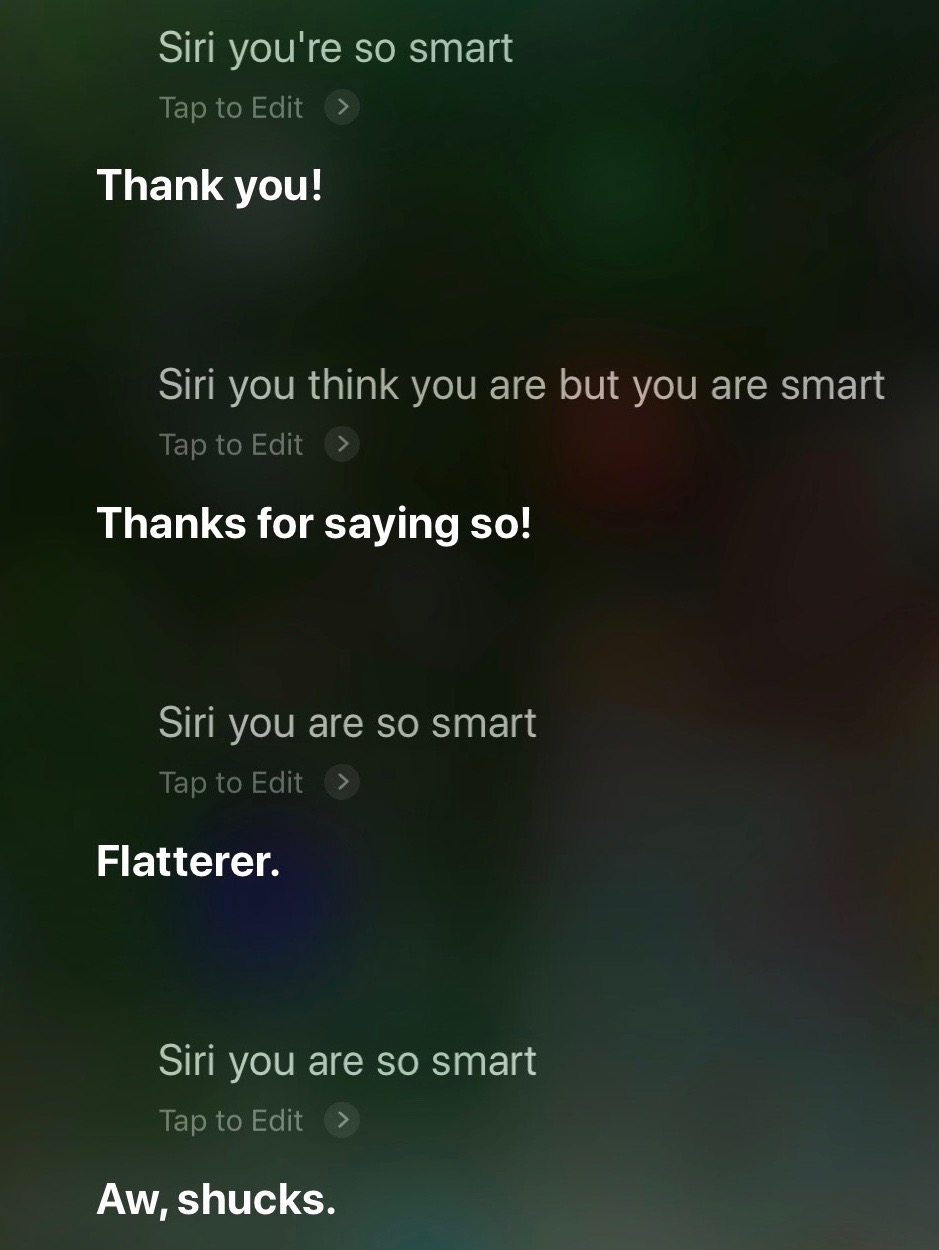
\includegraphics[height=0.7\textheight]{figures/siri_transcript.jpeg}
\end{center}
\end{frame}

\begin{frame}
\frametitle{AI Hype Distracts Us From ...}
\begin{itemize}
\item Having realistic expectations
\item Finding good business problems
\item Creating solutions that can be used by customers
\end{itemize}
\end{frame}

\begin{frame}
\frametitle{Don't Expect Too Much From AI}
\begin{itemize}
\item Data mining myth
\item Google search has trained us
\end{itemize}
\end{frame}

\begin{frame}
\frametitle{Good Business Problems Trump Technology}
\smartdiagramset{
	back arrow disabled=true,
}
\smartdiagram[flow diagram:verticall]{Problem,
  Data, AI}
\end{frame}


\end{document}